\documentclass[conference,10pt]{IEEEtran}
\IEEEoverridecommandlockouts
\usepackage{cite}
\usepackage{amsmath,amssymb,amsfonts}
\usepackage{graphicx}
\usepackage{textcomp}
\usepackage{xcolor}
\usepackage{url}
\usepackage{array}
\pdfinfo{
  /Title (Gini vs. Entropy: Does the Split Criterion Change Decision-Tree Interpretability on Medical Data?)
  /Author (Skye Fitzpatrick, Mark James Drohan, Aaron McGuinness, Mikey Fennelly)
}

\begin{document}

\title{Gini vs. Entropy: Does the Split Criterion Change Decision-Tree Interpretability on Medical Data?}

\author{
\IEEEauthorblockN{Skye Fitzpatrick}
\IEEEauthorblockA{\textit{University of Limerick}\\
Limerick, Ireland}
\and
\IEEEauthorblockN{Mark James Drohan}
\IEEEauthorblockA{\textit{University of Limerick}\\
Limerick, Ireland\\
24403342@studentmail.ul.ie}
\and
\IEEEauthorblockN{Aaron McGuinness}
\IEEEauthorblockA{\textit{University of Limerick}\\
Limerick, Ireland}
\and
\IEEEauthorblockN{Mikey Fennelly}
\IEEEauthorblockA{\textit{University of Limerick}\\
Limerick, Ireland}
}

\maketitle

\begin{abstract}
Gini impurity is the default split criterion in scikit-learn, yet its documentation gives no interpretability reason for preferring it to entropy. This paper asks whether the choice changes how interpretable a decision tree is, using the group's existing experiments on three UCI medical datasets. Four proxies are compared: tree size, test accuracy at fixed depth budgets, the stability of feature-importance rankings over 30 resamples, and node-by-node agreement of the depth-3 trees a clinician could read. No proxy favours one criterion on all three datasets. Accuracy gaps of one to seven test patients change sign across datasets and lie within the resolution of 60--114-patient test sets. On the two heart datasets, the readable trees share the root and both second-level splits, and differ only at the third level; on breast cancer, every threshold differs. The dataset moves Kendall's~$\tau$ about five times more than the criterion does. The depth limit matters more than the criterion: on each dataset the better depth-3 tree is at most two test patients short of the best setting tried. The paper recommends fixing the depth before the criterion and testing stability on held-out data.
\end{abstract}

\begin{IEEEkeywords}
decision trees, Gini impurity, information gain, interpretability, explanation stability, medical data
\end{IEEEkeywords}

\section{Introduction}
In the definition Molnar adopts, interpretability is the degree to which a human can understand the cause of a decision \cite{molnar2025}, and decision trees are usually counted among the models that meet it by construction. Molnar qualifies the claim: trees are very interpretable only while they stay short \cite{molnar2025}. Interpretability is therefore a property of a fitted tree, not of the model class, and any setting that changes the tree's shape can change it.

The split criterion is one such setting. The scikit-learn library grows trees with Gini impurity unless told otherwise and offers Shannon entropy as the alternative \cite{sklearnDTC}, but its documentation gives no reason to prefer either for interpretability. In healthcare the question has practical weight, because a review of 76 studies found that applications of explainable AI (XAI) to tabular health records rarely appraised the validity or robustness of their explanations \cite{caterson2024}.

This paper asks whether Gini or entropy changes the interpretability of decision trees trained on medical data. It reanalyses the group's recorded experiments on three UCI datasets, adds a node-by-node comparison of the depth-3 trees, and tests how far the measures support a verdict. Sections~II--V cover background, method, results with their critique, and conclusions.

\section{Background and Related Work}
\subsection{The Two Criteria}
For a node $m$ with class proportions $p_{mk}$, scikit-learn defines the two impurities as \cite{sklearnTree}
\begin{equation}
H_{\mathrm{Gini}}=\sum_k p_{mk}(1-p_{mk}),\qquad H_{\mathrm{ent}}=-\sum_k p_{mk}\log p_{mk}.
\end{equation}
Gini impurity equals $1-\sum_k p_{mk}^2$, the probability that a random case is misclassified when labelled at random according to the node's class proportions \cite{karabiber}. It comes from CART \cite{breiman2017}, while information gain, the drop in entropy, comes from ID3 \cite{quinlan1986}; CART is still usually paired with Gini and ID3 with entropy \cite{kavlakoglu2021}. The scikit-learn library implements both inside one optimised CART that builds binary trees \cite{sklearnTree}, so in this study the criterion is the only difference between the paired trees.

\subsection{How Often the Criteria Disagree}
Raileanu and Stoffel characterised formally when the two criteria select the same split. Across all possible databases with two binary attributes, a binary class and 50--200 rows, disagreement never exceeded 2\% of cases \cite{raileanu2004}. The group initially read this bound as a forecast of a null result. Its scope is narrower: it counts disagreements in the choice of a single split on small synthetic binary data, not differences in accuracy, and the authors add that specific databases may still differ significantly \cite{raileanu2004}. The features studied here are mostly continuous, so the bound does not transfer directly.

\subsection{What Makes a Tree Comprehensible}
In a study with 69 respondents, Piltaver \textit{et al.} found that more leaves clearly made trees harder to understand and that the depth of the leaf needed to answer a question had the largest effect, while tree depth on its own mattered little \cite{piltaver2016}. Terminal nodes multiply quickly with depth \cite{molnar2025}, which is why limiting \texttt{max\_depth} works as pre-pruning and why unpruned trees are hard to follow \cite{navlani2026}. Leaf count is therefore a better proxy than maximum depth.

\subsection{Instability}
Decision trees are unstable: small variations in the training set produce different trees, with changes in both accuracy and topology \cite{last2002}. The course readings agree \cite{molnar2025}, \cite{kavlakoglu2021}. An explanation that changes when a few patients are swapped is hard to trust, so stability is treated here as part of interpretability.

\section{Methodology}
\subsection{Datasets}
Table~\ref{tab:data} summarises the three datasets: Breast Cancer Wisconsin (Diagnostic) (BC) \cite{wolberg1993}, Heart Disease, Cleveland (HD) \cite{janosi1989} and Heart Failure Clinical Records (HF) \cite{uci2020hf}, \cite{chicco2020}. In HD, any disease grade from 1 to 4 counts as positive, following the usual Cleveland convention \cite{janosi1989}. HF's \texttt{time} column, the follow-up period \cite{uci2020hf}, was dropped because follow-up stops when a patient dies, so the column carries information about the outcome; Chicco and Jurman's main analyses also discard it \cite{chicco2020}.

\begin{table}[!t]
\caption{Datasets after preprocessing (Pos.: positive share of the training set)}
\label{tab:data}
\centering
\footnotesize
\setlength{\tabcolsep}{3pt}
\begin{tabular}{@{}l c c c >{\raggedright\arraybackslash}p{3.0cm}@{}}
\hline
 & Train/test & Feat. & Pos. & Preprocessing \\
\hline
BC & 455/114 & 30 & 37.4\% & Malignant $=1$; no other changes \\
HD & 242/61 & 22 & 45.9\% & \texttt{num}~$>0$ $=1$; \texttt{ca} median and \texttt{thal} mode imputed; 4 nominal features one-hot \\
HF & 239/60 & 11 & 32.2\% & \texttt{time} removed \\
\hline
\end{tabular}
\end{table}

\subsection{Matched Training}
Each dataset was split once, stratified 80/20, with \texttt{random\_state}~$=42$, and the Gini and entropy trees were trained on the same split with identical settings. Fixing the seed matters because scikit-learn permutes features at every split and breaks tied improvements at random \cite{sklearnDTC}.

\subsection{Interpretability Proxies}
\textit{Structure:} depth, leaves, nodes and distinct features used by the unconstrained trees. \textit{Accuracy at fixed complexity:} test accuracy with \texttt{max\_depth} set to 3, 5, 7 and 10. \textit{Stability:} the data were re-split 30 times (\texttt{random\_state}~$=$~run, tree seed fixed), an unconstrained tree was trained on each training portion, and its impurity-based importances were ranked. Each later run was compared with run 0 by Kendall's~$\tau$ over the full ranking and by the Jaccard overlap of the top five features, and the 29 values were averaged. \textit{Readable levels:} the depth-3 trees were compared at their seven split positions, counting positions with the same feature and threshold.

\subsection{Existing Results Only}
The group chose to analyse its recorded runs without re-running them. Patient counts, the binomial standard error $\sqrt{p(1-p)/n}$, gaps and split counts were derived from the notebook outputs and tree plots, which accompany this paper with the derivation script.

\section{Results and Discussion}
\subsection{Structure}
Table~\ref{tab:struct} shows no consistent structural winner. Gini trees are one level shallower on HD and HF but deeper on BC. Entropy has fewer or equal leaves everywhere, but only BC shows a material gap, 17 against 24. Node counts add nothing: every tree is binary, so nodes $=2\times\text{leaves}-1$ in all six cases. Since more leaves clearly reduce comprehension \cite{piltaver2016}, trees with 17--51 leaves make poor reading whichever criterion grew them.

\begin{table}[!t]
\caption{Unconstrained trees on the single 80/20 split}
\label{tab:struct}
\centering
\footnotesize
\begin{tabular}{@{}l l c c c c@{}}
\hline
 & Criterion & Correct (\%) & Depth & Leaves & Features \\
\hline
BC & Gini & 106/114 (93.0) & 8 & 24 & 14 \\
   & Entropy & 109/114 (95.6) & 7 & 17 & 12 \\
HD & Gini & 46/61 (75.4) & 9 & 48 & 15 \\
   & Entropy & 47/61 (77.0) & 10 & 48 & 16 \\
HF & Gini & 43/60 (71.7) & 13 & 51 & 9 \\
   & Entropy & 36/60 (60.0) & 14 & 50 & 9 \\
\hline
\end{tabular}
\end{table}

\subsection{Accuracy at a Fixed Depth}
Fig.~\ref{fig:depth} expresses the accuracy gap in test patients. Entropy is ahead by 2--4 patients on BC at every depth, Gini by 2--6 on HF, and HD changes sign. These gaps must be read against the resolution of the test sets: one patient is worth 0.88 percentage points on BC and about 1.6 on HD and HF, and the binomial standard error of a single accuracy is 1.9--6.3 points. HF's largest gap, 6 patients or 10 points, is under twice the standard error of one estimate. Both criteria are scored on the same patients, so a paired test such as McNemar's is needed, but per-patient predictions were not recorded; the paper therefore does not rank the criteria on accuracy.

\begin{figure}[!t]
\centering
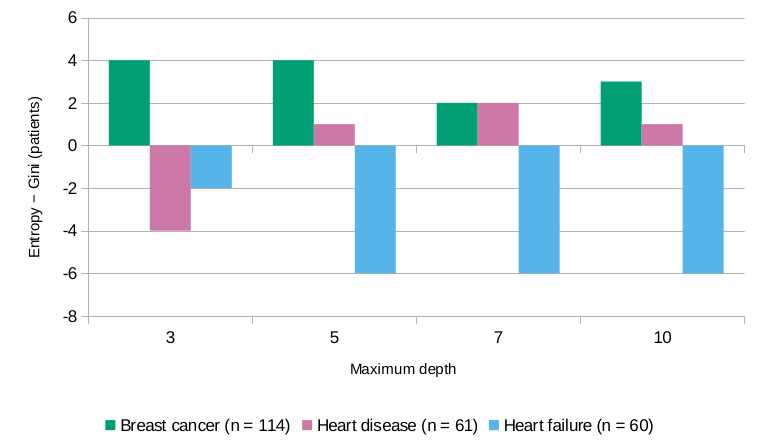
\includegraphics[width=\columnwidth]{fig-depth-gap.png}
\caption{Accuracy gap at fixed depth: entropy minus Gini, in correctly classified test patients (positive favours entropy).}
\label{fig:depth}
\end{figure}

Depth gives a clearer signal. The depth-3 trees are the best setting tried on HD (Gini, 53/61) and HF (Gini, 47/60), and on BC the depth-3 entropy tree is two patients short of the best (107 against 109). The readable tree costs almost nothing measurable, while depth moves accuracy as much as the criterion does: HD Gini drops from 53 to 44 correct between depths 3 and 5.

\subsection{The Readable Levels}
Table~\ref{tab:splits} compares the depth-3 trees node by node. On HD and HF the two criteria give the same root and the same two second-level splits, feature and threshold; they diverge only at the third level, at two positions on HD and one on HF. On HF both trees begin with serum creatinine and then ejection fraction, the two features Chicco and Jurman identified as most relevant to survival \cite{chicco2020}, which suggests the top of the tree reflects the data rather than the criterion.

\begin{table}[!t]
\caption{Agreement of the depth-3 trees (Gini vs. entropy)}
\label{tab:splits}
\centering
\footnotesize
\setlength{\tabcolsep}{3pt}
\begin{tabular}{@{}l c c c >{\raggedright\arraybackslash}p{3.1cm}@{}}
\hline
 & Splits & Identical & Same feat. & First difference \\
\hline
BC & 7/6 & 0 of 6 & 3 of 6 & Root: \texttt{perimeter3} $\le$ 112.8 vs. $\le$ 114.45 \\
HD & 7/7 & 5 of 7 & 5 of 7 & Level 3: \texttt{ca} vs. \texttt{chol}; \texttt{age} vs. \texttt{thalach} \\
HF & 6/6 & 5 of 6 & 5 of 6 & Level 3: \texttt{serum\_sodium} vs. \texttt{platelets} \\
\hline
\multicolumn{5}{@{}p{\columnwidth}@{}}{\scriptsize Identical: same feature and threshold at a position where both trees split.}
\end{tabular}
\end{table}

BC behaves differently. Both roots split on \texttt{perimeter3}, but at different thresholds, so 297 training patients go left under Gini and 308 under entropy; every node below then sees different data, and no threshold matches. This explains why 10 of 19 shared positions agree exactly, well below the 98\% that Raileanu and Stoffel's bound might suggest \cite{raileanu2004}: their bound concerns one decision on fixed data, whereas in a tree one early disagreement changes the data for every descendant. Small differences still move accuracy: on HD, two differing bottom splits separate 53 from 49 correct.

\subsection{Stability of Importance Rankings}
Fig.~\ref{fig:stab} shows that the dataset, not the criterion, sets stability. The largest gap between criteria is 0.058 in $\tau$ and 0.126 in Jaccard, and its sign changes across datasets, whereas $\tau$ spans 0.275--0.303 across datasets for a fixed criterion and Jaccard 0.311--0.464. BC, with 30 features of which 12--14 are used, ranks least consistently.

\begin{figure}[!t]
\centering
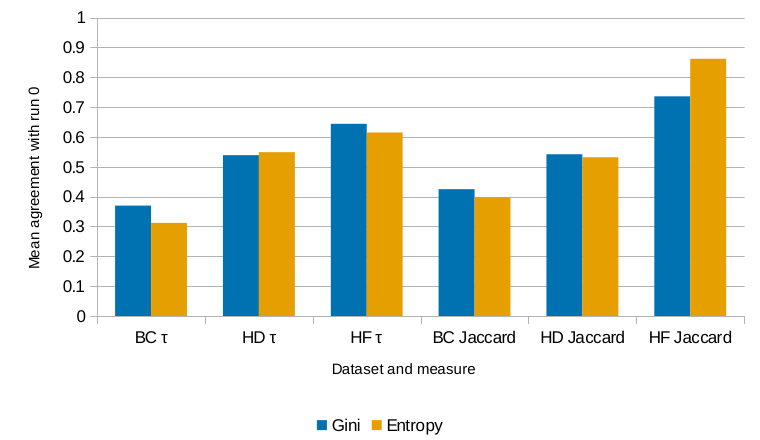
\includegraphics[width=\columnwidth]{fig-stability.png}
\caption{Stability over 30 resamples: mean Kendall's $\tau$ and top-5 Jaccard overlap of each run's importance ranking with run 0.}
\label{fig:stab}
\end{figure}

The measure itself limits what Fig.~\ref{fig:stab} can show. Every comparison is made against run 0, so an unusual first split shifts all 29 values together, and no spread is reported. The importances are impurity-based and computed on the training portion of unconstrained trees, and the scikit-learn documentation warns that such importances can rate features highly that do not predict unseen data when the model overfits, and that they favour high-cardinality features \cite{sklearnPI}; Molnar recommends estimating importance on held-out data for the same reason \cite{molnar2025}. HD's one-hot binary columns are exposed to that bias. Finally, the stability measured is that of the 33--101-node trees, not of the depth-3 trees that Table~\ref{tab:splits} shows a reader would use.

\subsection{Hypotheses}
H1 (Gini gives simpler trees with less stable rankings) is not supported: Gini is shallower on two datasets, has more leaves on BC, and has the higher $\tau$ on BC and HF. H2 (entropy gives more stable rankings but deeper trees) is not supported either: entropy is deeper on two datasets but more stable in $\tau$ on HD only. H3 (dataset dependence) is supported: the dataset dominates stability and decides which criterion appears ahead on accuracy. H0 is accepted: the only measure that leans the same way on all three datasets is leaf count, and its margin there is 0 and 1 leaves on two of them. No proxy was checked against human judgement, and comprehension depends on the reader's question \cite{piltaver2016}.

\section{Conclusion and Limitations}
On these datasets the split criterion does not change interpretability in any consistent way. Structural size differs by one level and up to seven leaves without a pattern (RQ1). No criterion gives more accuracy per unit of depth once test-set resolution is considered, though on each dataset the better depth-3 tree matches or nearly matches the best setting tried (RQ2). Stability is driven by the dataset, and the criterion effect changes sign (RQ3). The readable top levels agree exactly on the two heart datasets and diverge from the root on breast cancer, where a small threshold shift cascades through the tree (RQ4).

The analysis leaves several questions open. Accuracy rests on one split with no paired test, so small real differences cannot be excluded. The stability measure does not measure the stability of a readable explanation. Split agreement was read from plots at depth 3 only. Only \texttt{max\_depth} pruning was used; cost-complexity pruning, other criteria and ensembles were not studied. The datasets come from one domain, and no clinician judged any tree, so every conclusion concerns proxies for interpretability rather than interpretability itself.

Four changes would address these limits. Practitioners should choose the depth budget first. Accuracy should be reported in patients with paired tests over many resamples. Stability should be measured pairwise on the depth-limited trees, using permutation importance on held-out data. A small clinician study of paired depth-3 trees would show whether the divergences in Table~\ref{tab:splits} change what readers conclude.

\clearpage
\label{paper:references}
\bibliographystyle{IEEEtran}
\bibliography{refs}

\end{document}
